\chapter{Simulation und Ergebnisse}
\label{kap:editor-ergebnisse}

\section{Simulieren}

\tasten{Strg}{R} sichert die Datei und startet \esim. Während der Rechnung
zeigt die Statuszeile Analyse und Fortschritt in Prozent, das
\menue{Protokoll} die Ausgabe des Simulators. \tasten{Strg}{.} bricht ab.
Nach dem Ende erscheinen die Ergebnisse; die Auswahl von Analyse, Größen und
Zoom bleibt über neue Läufe hinweg erhalten, sodass man nach einer Änderung
direkt vergleichen kann.

Die Ergebnisdateien liegen in einem temporären Ordner des Editors. Wer die
CSV-Dateien weiterverwenden will, rechnet dieselbe Datei auf der
Kommandozeile (Kapitel~\ref{kap:kommandozeile}) oder aus Python.

\section{Das Ergebnisfeld}

\begin{figure}[htbp]
  \centering
  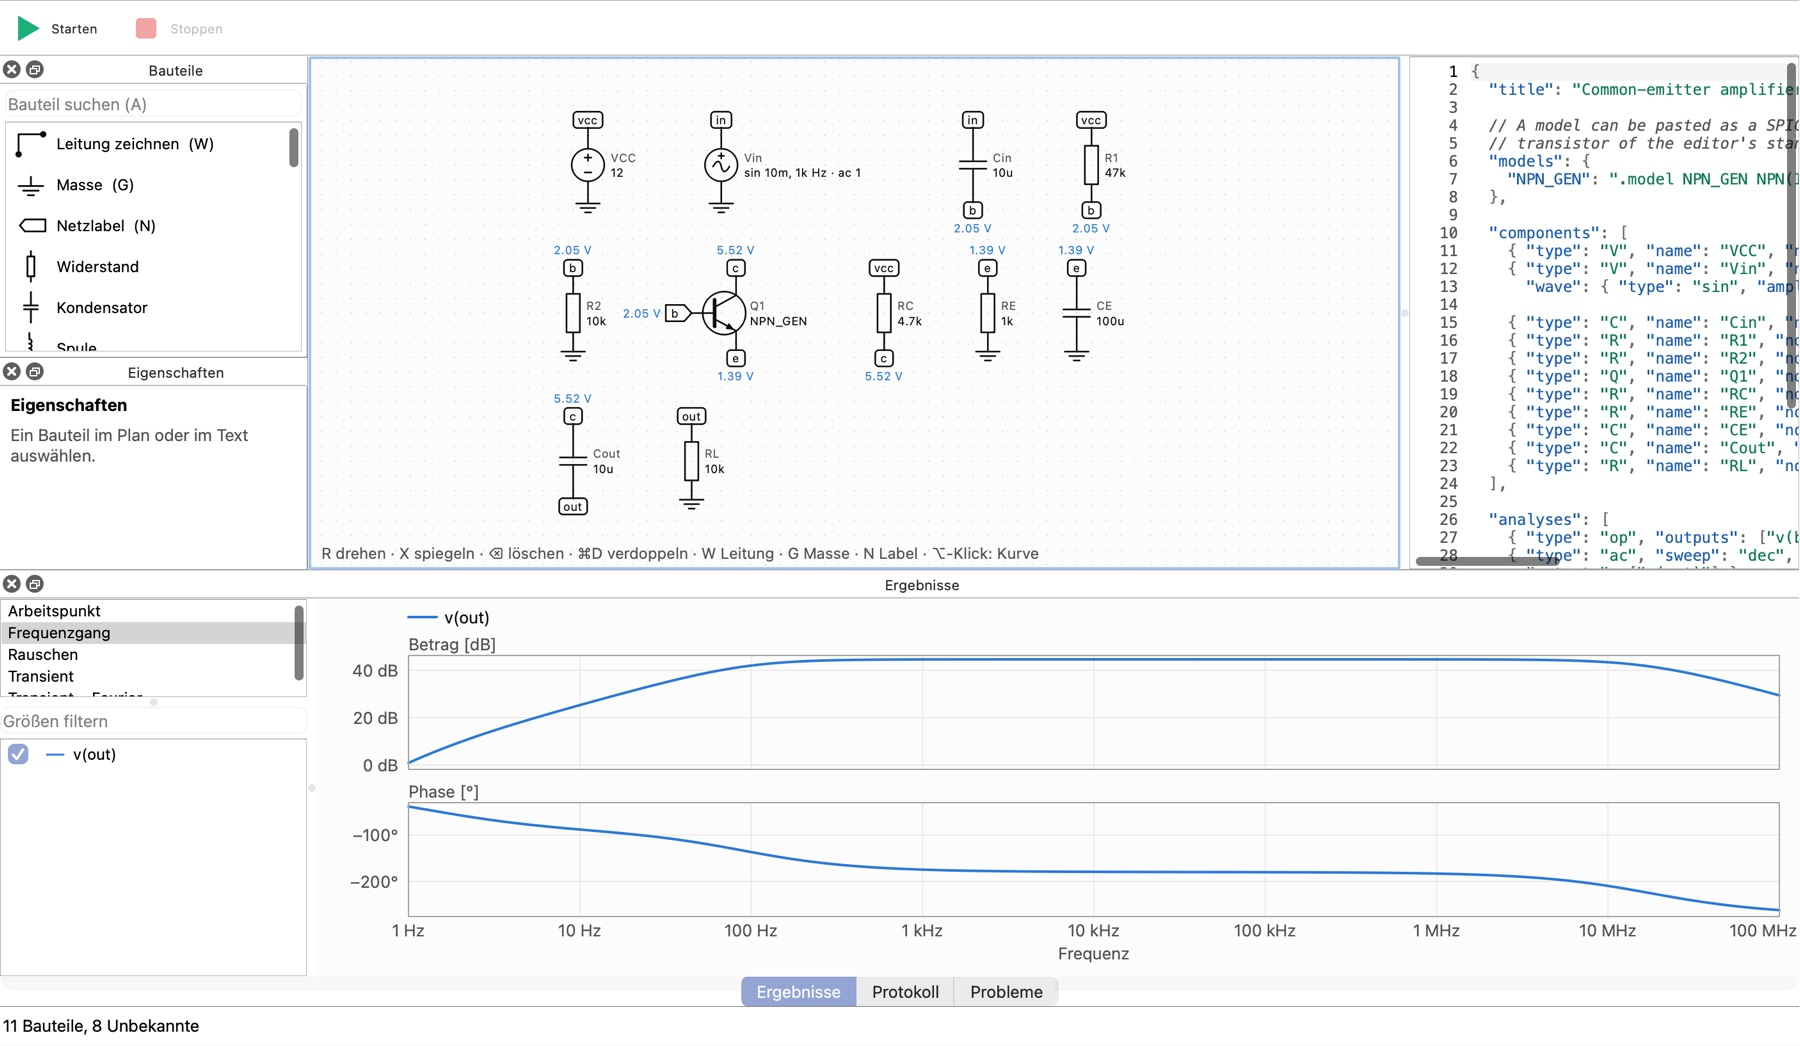
\includegraphics[width=\textwidth]{bjt_amplifier.jpg}
  \caption{Emitterschaltung (\code{examples/bjt_amplifier.json}) nach der
    Simulation: Spannungen des Arbeitspunkts an den Labels, unten der
    Frequenzgang als Betrag in dB und Phase.}
  \label{abb:bjt}
\end{figure}

Links oben steht die Liste der \textbf{Analysen} der Datei, mit deutschen
Namen (\menue{Arbeitspunkt}, \menue{DC-Sweep}, \menue{Frequenzgang},
\menue{Transient}, \menue{Periodischer Zustand}, \menue{Rauschen},
\menue{Empfindlichkeit}, \menue{Anpassung}). Benannte Analysen tragen
ihren Namen, Studien den Zusatz »(Sweep)« oder »(Monte Carlo)«. Haben
Analysen Messgrößen über viele Läufe oder eine Fourier-Analyse, kommen
Einträge »– Messgrößen« und »– Fourier« hinzu.

Darunter die \textbf{Größen} der gewählten Analyse mit Häkchen, ein Feld zum
Filtern (z.\,B. »v(« für alle Spannungen) und die \textbf{Wertetabelle}:
Arbeitspunkt, Messgrößen, Statistik der Rechnung (Schritte, Iterationen,
Ereignisse) und bei Monte Carlo Mittelwert, Streuung, Minimum und
Maximum. Eine Messung ohne Ergebnis steht als »nicht bestimmt« darin.

Rechts die \textbf{Kurven}.

\section{Kurven}

Die Kurven einer Analyse stehen in übereinanderliegenden Feldern mit
gemeinsamer $x$-Achse:

\begin{itemize}
  \item \textbf{Zeitverläufe} und \textbf{DC-Sweeps}: ein Feld für
    Spannungen, eines für Ströme, eines für alle übrigen Größen.
  \item \textbf{Frequenzgänge}: Betrag in dB und Phase in Grad über
    logarithmischer Frequenz.
  \item \textbf{Rauschen}: die Rauschdichten über der Frequenz.
  \item \textbf{Sweeps}: eine Kurve je Parameterwert in Stufen einer
    Blauskala; die Legende nennt die Werte.
\end{itemize}

\begin{center}
\begin{tabularx}{\textwidth}{@{}P{5.2cm}L@{}}
  \toprule
  Bedienung & Wirkung \\
  \midrule
  Mausrad, Touchpad auf/ab, spreizen & Zoomt in $x$ um den Mauszeiger. \\
  \taste{Strg} + Mausrad & Zoomt in $y$ im Feld unter dem Mauszeiger. \\
  Touchpad seitwärts & Verschiebt in $x$. \\
  Ziehen mit der Maus & Zoomt auf das aufgezogene Rechteck. \\
  Doppelklick, \tasten{Strg}{0} & Zeigt alles. \\
  Maus über den Kurven & Fadenkreuz mit den Werten aller Kurven an dieser Stelle. \\
  Rechtsklick & \menue{Alles zeigen}, \menue{Als Bild speichern \dots} (PNG). \\
  \bottomrule
\end{tabularx}
\end{center}

Beim Zoomen in $x$ passt sich die $y$-Achse jedes Felds dem sichtbaren
Ausschnitt an. Die Kurven werden je Bildpunkt auf Minimum und Maximum
verdichtet; auch Millionen von Punkten bleiben deshalb flüssig und ohne
verschluckte Spitzen.

\paragraph{Kurven aus dem Plan.}
\tasten{Alt}{Klick} auf eine Leitung zeigt deren Spannung, auf ein Bauteil
dessen Strom, ebenso \menue{Spannung v(…) zeigen} und \menue{Strom i(…)
zeigen} im Kontextmenü. Der Editor zeigt die Größe in einer Analyse, die
sie enthält, und hakt sie an. Gespeichert sind nur Größen, die unter \code{"outputs"}
stehen (oder alle, wenn die Datei kein \code{"outputs"} hat).

\section{Messgrößen über viele Läufe}

Analysen mit \code{monte_carlo} oder \code{param_sweep} liefern ihre
Messgrößen je Lauf. Der Eintrag »– Messgrößen« zeigt sie in eigenen
Darstellungen, gewählt über \menue{Darstellung} und je Analyse gemerkt.

\subsection*{Monte Carlo: Histogramm}

Jede Messgröße bekommt ein eigenes Feld mit eigener Achse
(Abbildung~\ref{abb:mc}). Die Klassenbreite folgt der Regel von
Freedman und Diaconis. Der Mittelwert ist als Linie, der Bereich $\pm\sigma$
als Fläche markiert; die Kopfzeile nennt Anzahl $n$, Mittelwert $\mu$,
Standardabweichung $\sigma$, die relative Streuung $\sigma/\mu$, Minimum und
Maximum. Fährt die Maus über eine Klasse, zeigt ein Tooltip deren Bereich
und wie viele Läufe (und wie viel Prozent) hineinfallen. Ein Rechtsklick
sichert das Histogramm als Bild.

\begin{figure}[htbp]
  \centering
  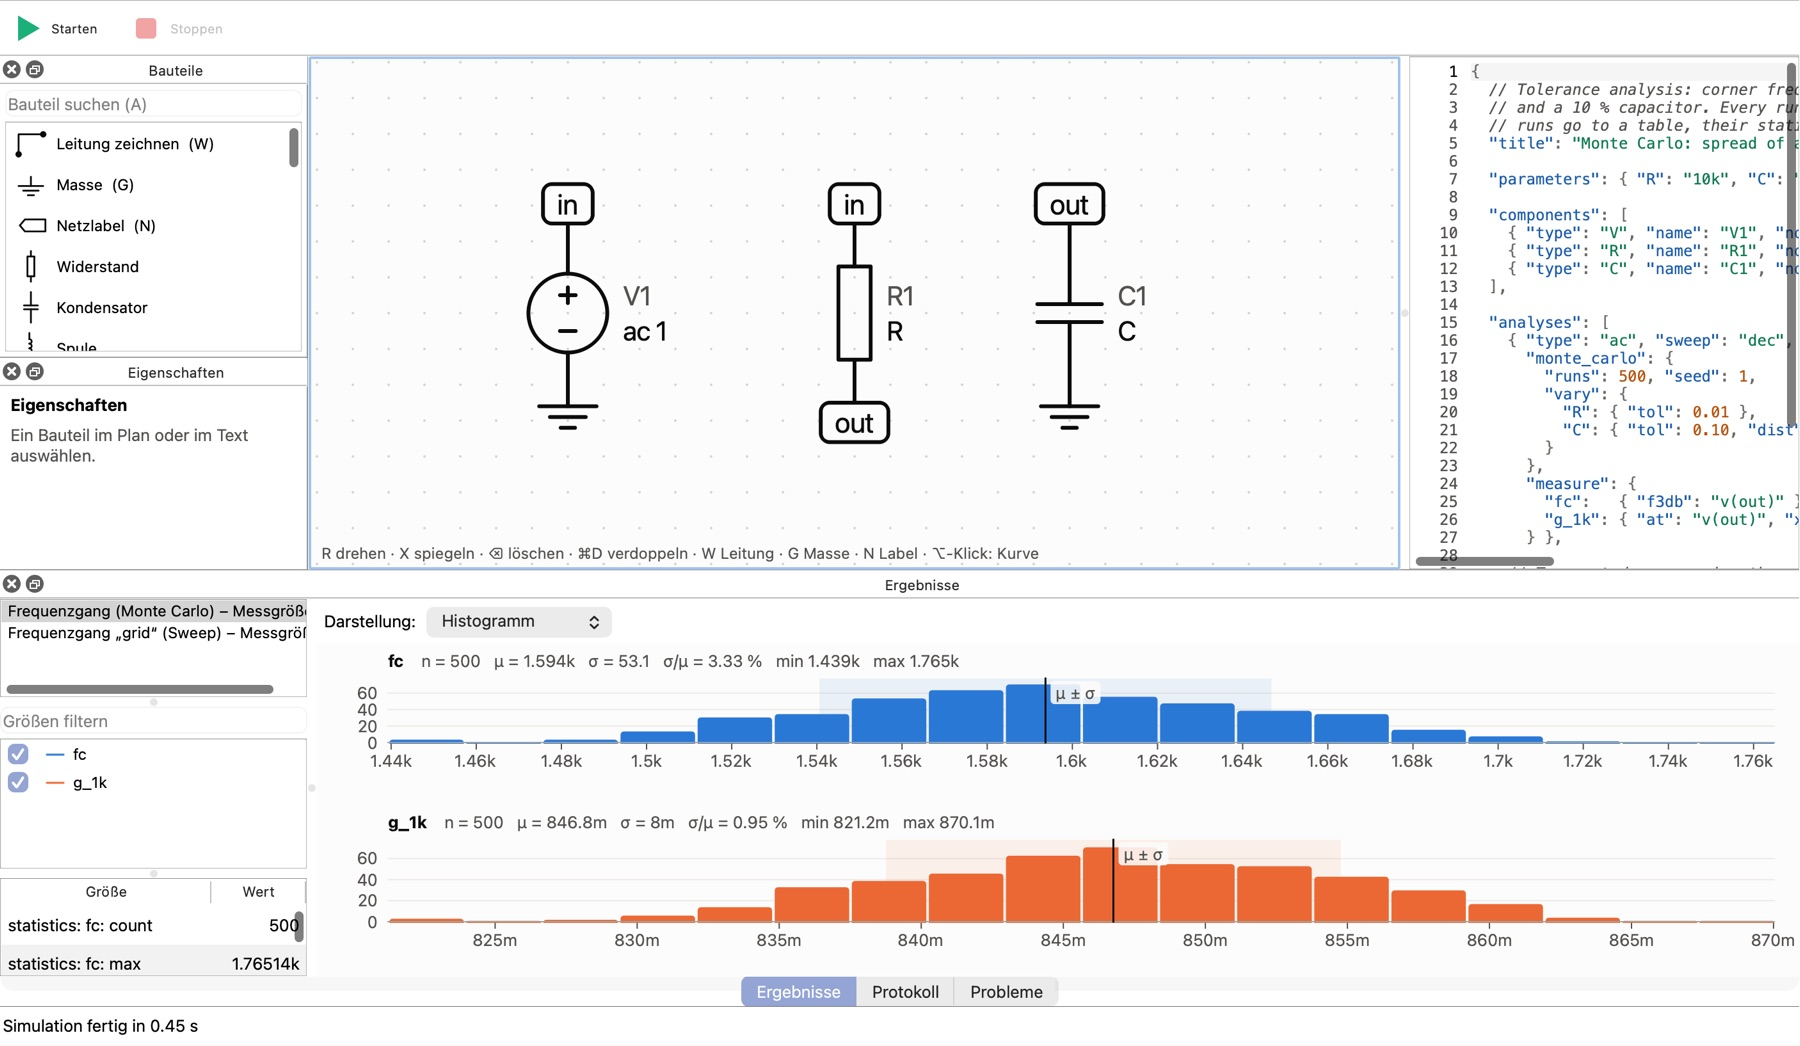
\includegraphics[width=\textwidth]{monte_carlo_filter.jpg}
  \caption{Monte-Carlo-Analyse eines RC-Filters
    (\code{examples/monte_carlo_filter.json}): 500 Läufe mit gestreutem $R$
    und $C$, Histogramme der Grenzfrequenz und der Verstärkung bei 1\,kHz.}
  \label{abb:mc}
\end{figure}

\subsection*{Monte Carlo: Streuung über einem Parameter}

\menue{Streuung über \textit{p}} zeigt jede Messgröße als Punktwolke über
dem gezogenen Wert des Parameters $p$. Daran sieht man, welcher Parameter
die Streuung verursacht: Eine schräge, schmale Wolke bedeutet starken
Einfluss, eine waagrechte keinen.

\subsection*{Sweeps: Kennlinie über dem Parameter}

Bei Parameter-Sweeps zeigt \menue{über \textit{p}} jede Messgröße als Linie
mit Punkten über dem Parameter, über mehrere Dekaden logarithmisch. Bei
verschachtelten Sweeps ergeben die weiteren Parameter eine Kurvenschar auf
der Blauskala – etwa die Periode eines Oszillators über $C$ für mehrere
Werte von $R$.

\section{Ein Beispiel mit Ereignissen}

\begin{figure}[htbp]
  \centering
  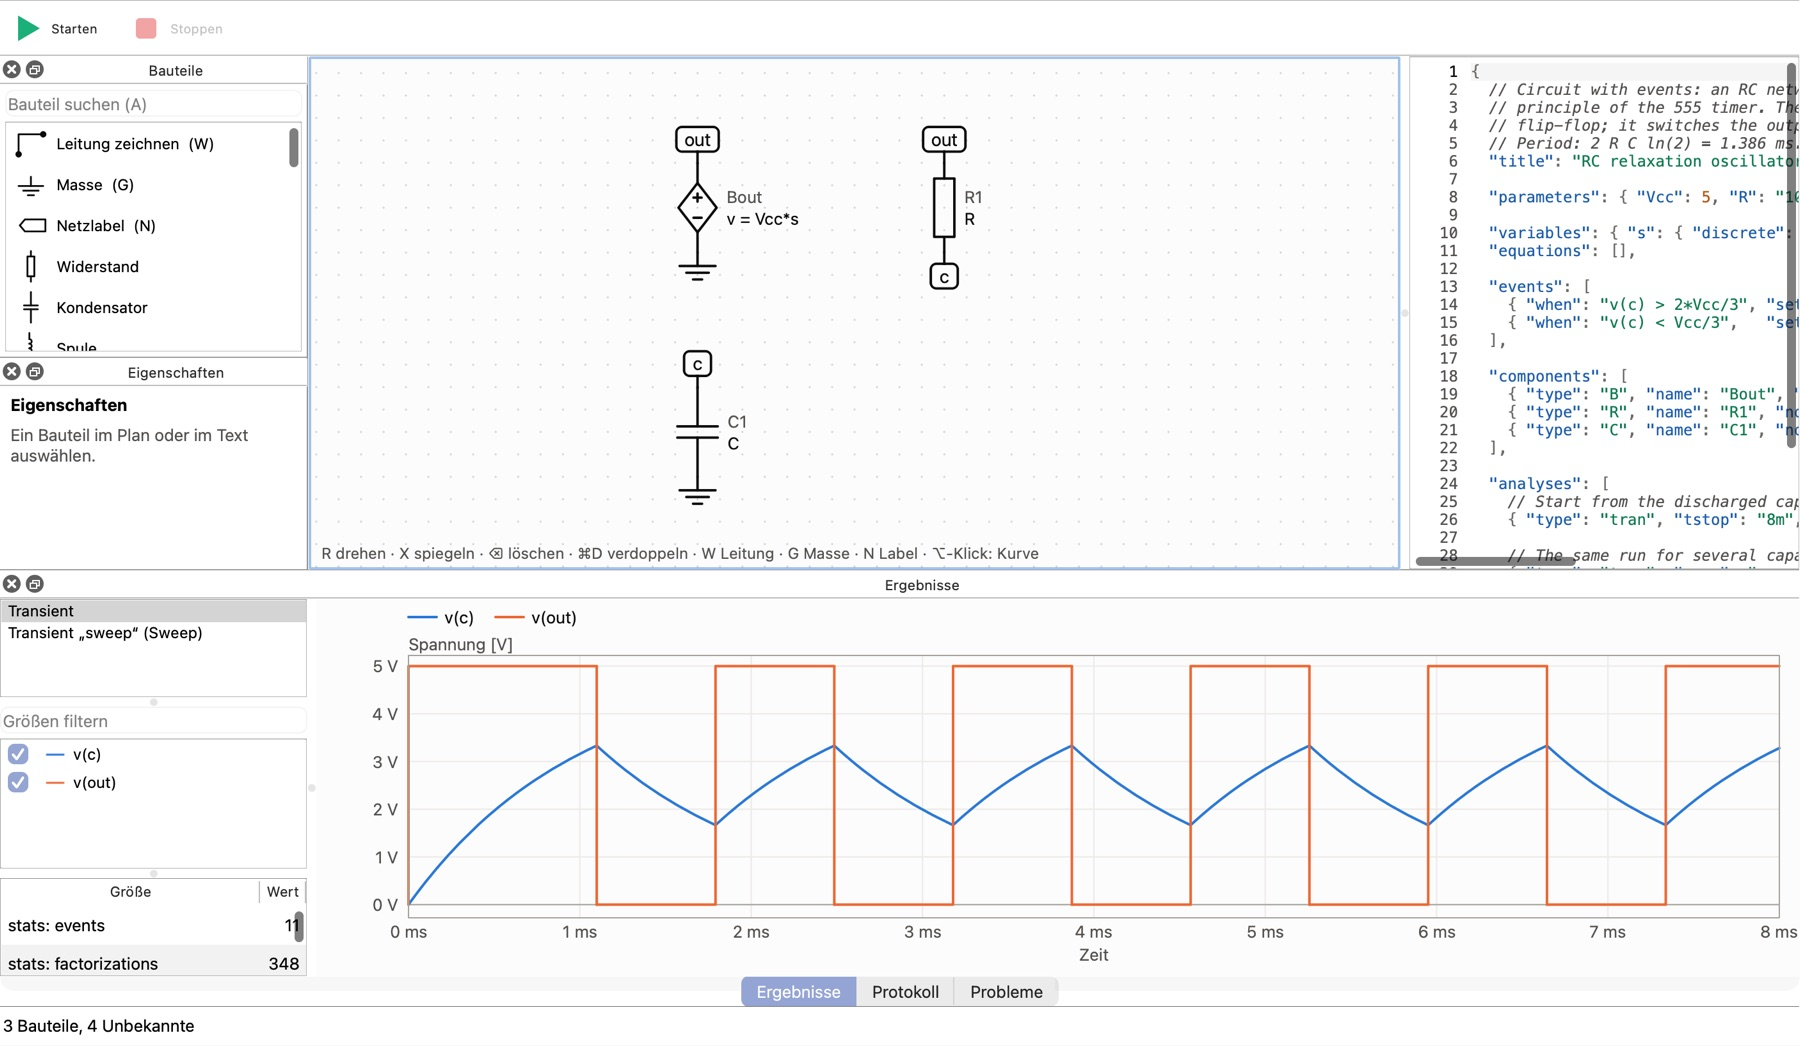
\includegraphics[width=\textwidth]{relaxation_oscillator.jpg}
  \caption{Kippschwinger nach dem Prinzip des 555
    (\code{examples/relaxation_oscillator.json}): Eine Verhaltensquelle
    schaltet über eine diskrete Variable \code{s}, die zwei Ereignisse
    setzen. Die Umschaltzeitpunkte sind exakt bestimmt.}
  \label{abb:relax}
\end{figure}

Abbildung~\ref{abb:relax} zeigt eine Schaltung ohne Schaltplan-Leitungen:
Die Datei hat keinen gezeichneten Plan, der Editor hat jedes Bauteil mit
Labels an den Anschlüssen angeordnet. Das Beispiel enthält außerdem einen
Sweep über $C$, dessen Kurvenschar unter »Transient „sweep“ (Sweep)«
erscheint.
